\documentclass[11pt]{report}
\usepackage[latin1]{inputenc} 
\usepackage[T1]{fontenc}

\usepackage{amsmath,amssymb,amscd,amsfonts,verbatim}
\usepackage{IEEEtrantools,mathrsfs}
\usepackage{tikz,color}

\oddsidemargin 0mm
\evensidemargin 0mm
\textwidth 160mm
\topmargin -20mm
\textheight 220mm

\parindent 0pt
\pagestyle{empty}
\def\baselinestretch{1.2}

\usepackage[a4paper,top=2.5cm,bottom=2.5cm,left=2.5cm,right=2.5cm]{geometry}

\def\R{\mathbb{R}}
\def\calA{\mathcal{A}}
\def\2toro{\mathbb{T}^2}
\def\trasl2toro{\overline{\mathbb{T}}^2}

\begin{document}
\centerline{\bf\large Integration of $1/\delta_h$}
\vskip 0.5cm

We describe the explicitly computation of the integral of
$1/{\delta_h}$ over $$\2toro = \{(\ell',\ell): -\pi \leq \ell' \leq
\pi, -\pi \leq \ell\leq \pi\},$$ assuming that $(\ell'_h,\ell_h)$ is
an internal point of this domain.
%
First, we move the point $(\ell'_h,\ell_h)$, corresponding to the
local minimum value $d_h$, into the origin of the reference system by
the variable change
%
\begin{equation}
  \sigma_h: \ \2toro \ni (\ell',\ell) \mapsto 
  (\ell'-\ell'_h,\ell-\ell_h) =: \kappa = (k',k) \in \trasl2toro
  \label{eq:translation}
\end{equation}
%
where we set $\trasl2toro = \sigma_h\left(\2toro\right)$. The matrix
%
\begin{equation} 
  {\cal T} = \left[\begin{array}{cc} \displaystyle\frac{1}{\rho_1} &
      -\displaystyle\frac{\rho_2}{\rho_1\rho_4}\cr & \cr
      0 & \displaystyle\frac{1}{\rho_4} \end{array}\right], 
  \quad \rm{with}\quad
  \rho_1 = |\tau'|, \quad \rho_2  =
  -\frac{\langle\tau',\tau\rangle}{|\tau'|}, \quad \rho_4 = 
  \frac{\sqrt{\det(\calA_h)}}{|\tau'|},
\end{equation}
is such that
\begin{equation}
{\cal T}^t{\calA_h}{\cal T} = {\cal I}_2\ .
%\label{diagonalization}
\end{equation}
Then, the following coordinate change
\begin{equation}
\mathfrak{R}: \kappa \mapsto \psi = {\cal R} \,\kappa\,,\qquad\mbox{with}\qquad
{\cal R} = {\cal T}^{-1} = \left[\begin{array}{cc} 
\rho_1 & \rho_2 \cr 0 & \rho_4 \cr \end{array}\right]\ ,
\label{eq:invlinelim}
\end{equation}
brings $\delta_h^2\circ\sigma_h^{-1}$ into the form
\begin{equation}
  \delta_h^2\circ\sigma_h^{-1}\circ\mathfrak{R}^{-1}(\psi) = y'^2 + y^2 + d_h^2\,,
  \hskip 1cm \psi=(y',y)
\label{eq:delta_h}
\end{equation}
and transforms the domain $\trasl2toro$ into a parallelogram with two
sides parallel to the $y$ axis (see Figure~\ref{coord_change}).

\begin{figure}[b]
%\centerline{\psfig{figure=./figures/averaging/coord_change2.eps,width=10cm}}
%\includegraphics{}
 \centering
 \begin{tikzpicture}[scale=0.7]
% assi cartesiani 1
   \draw[->,thin] (-9.5,0) -- (-4,0) node[below] {$\ell'$};
   \draw[->,thin] (-7,-3) -- (-7,3) node[left] {$\ell$}; \node at
   (-7.4,-0.3) {$O$};
% assi cartesiani 2
   \draw[->,thin] (-3,0) -- (2,0) node[below] {$k'$}; \draw[->,thin]
   (0,-3) -- (0,3) node[left] {$k$}; \node at (-0.3,-0.3) {$O$};
% assi cartesiani 3
   \draw[->,thin] (3,0) -- (10,0) node[below] {$y'$}; \draw[->,thin]
   (7,-3) -- (7,3) node[left] {$y$}; \node at (6.7,-0.3) {$O$};
% rettangolo 1
   \draw (-5.5,1.5) -- (-8.5,1.5) -- (-8.5,-1.5) -- (-5.5,-1.5) --
   cycle; \node at (-6.2,2) {$\2toro$}; \draw[dashed] (-6,0)
   node[below] {$\ell'_h$} -- (-6,1) -- (-7,1) node[left]
   {$\ell_h$}; \node at (-6,1) {$\bullet$};
% rettangolo 2
   \draw (0.5,0.5) -- (-2.5,0.5) -- (-2.5,-2.5) -- (0.5,-2.5) --
   cycle; \node at (-1.3,1.1) {$\trasl2toro$};
% rettangolo 3
   \draw (9.5,1) -- node[above] {$r_2$} (5.5,1) -- node[left] {$r_3$}
   (3.5,-1.5) -- node[below] {$r_4$} (7.5,-1.5) -- node[right] {$r_1$}
   (9.5,1); \node at (5.5,1.5) {$\mathfrak{R}[\trasl2toro]$};
% trasformazioni
   \draw[->] (-5.5,2) .. controls (-4,3) .. (-2,1.5); \node at (-4,3)
   {$\sigma_h$}; \draw[->] (1,1.5) .. controls (3,3) .. (4.5,2); \node
   at (3,3) {$\mathfrak{R}$};
      \end{tikzpicture}
  \caption{Description of the transformations of the integration
    domain $\2toro$ with the two coordinate changes
    \eqref{eq:translation}, \eqref{eq:invlinelim}.}
%  used to bring the squared Wetherill function ${\rm d}^2(\ell,\ell')$
%  into the form $y^2 + y'^2 + {(d^+_{min})}^2$ in the new variables
%  $(y',y)$. Note that $\overline\ell'=0$ implies that $\trasl2toro$ is
%  symmetric with respect to the $k$ axis
  \label{coord_change}
\end{figure}

Using the variable changes \eqref{eq:translation}, \eqref{eq:invlinelim} and
the polar coordinates map $\mathfrak{P}$, with inverse
%
\begin{displaymath}
\mathfrak{P}^{-1}: (r,\theta)\mapsto (y_1, y_2) = (r \cos\theta, r
\sin\theta)
\end{displaymath}
%
we obtain
%
%\begin{IEEEeqnarray}{rCl}
\begin{equation}
  \int_{\2toro} {1\over {\delta_h}}\,d\ell'\,d\ell = \frac{1}
  {\sqrt{\det({\calA_h})}} \int_{{\mathfrak{R}}[\trasl2toro]}
  \frac{1}{\sqrt{y'^2+y^2 + d_h^2}}\,d y'\,d y =
  \frac{1}{\sqrt{\det({\calA_h})}} \int_{{\cal D}_h} \frac{r}{\sqrt{r^2 +
      d_h^2}}\,d r\,d \theta
\label{approx_integral}
\end{equation}
%\end{IEEEeqnarray}
%
where $\mathfrak{R}^{-1}\left[\mathfrak{P}^{-1}\left({{\cal
        D}_h}\right)\right] = \trasl2toro$.
%
Then, we decompose the domain ${\cal D}$ into four parts 
%
$$
\mathfrak{T} = \bigcup_{j=1}^4 \left\{(r,\theta)\in \R^2 \ :\
\theta_j\leq \theta \leq \theta_{j+1} \hbox{ and }\ 0\leq r\leq
r_j(\theta) \right\}
$$
%
where $r_j(\theta)$, with $j=1\dots 4$, represent the lines ${\rm
  r}_j$ delimiting $\mathfrak{R}[\trasl2toro ]$ (see
Figure~\ref{parall_splitting}) and in polar coordinates are given
by
\begin{equation*}\begin{matrix}
    r_1(\theta)=\displaystyle\frac{\rho_1 \rho_4 (\pi-\ell'_h)}{\rho_4
      \cos \theta -\rho_2 \sin \theta}\ , & \qquad &
    r_2(\theta)=\displaystyle\frac{\rho_4 (\pi-\ell_h)}{\sin \theta}\ ,\\ & & \\
    r_3(\theta)=\displaystyle\frac{-\rho_1 \rho_4
      (\pi+\ell'_h)}{\rho_4 \cos \theta -\rho_2 \sin \theta}\ , &
    \qquad & r_4(\theta)=\displaystyle\frac{-\rho_4
      (\pi+\ell_h)}{\sin \theta}\ .\\
\end{matrix}	
\end{equation*}
While $\theta_1 = \theta_5 -2\pi$ and $\theta_{j+1}$ are the
counter-clockwise angles between the $y'$-axis and the vertexes $v_l$
seen from the origin of the axes (see Figure~\ref{parall_splitting}):
$$
0 < \theta_2 < \theta_3 < \pi < \theta_4 < \theta_5 < 2\pi\ .
$$

\begin{figure}[t]
  \centering
% \includegraphics[scale=0.3]{Figure/dec_ell}
 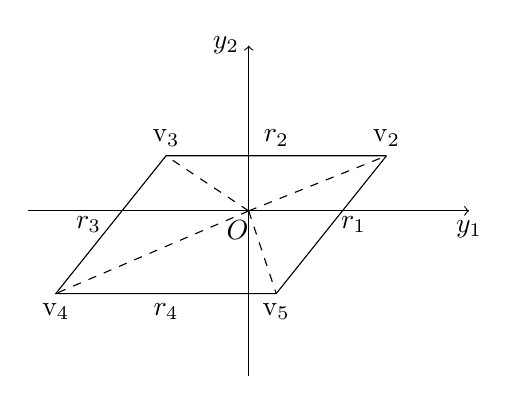
\begin{tikzpicture}[scale=0.7]
% assi cartesiani 2
   \draw[->,thin] (-4,0) -- (4,0) node[below] {$y_1$}; \draw[->,thin]
   (0,-3) -- (0,3) node[left] {$y_2$}; \node[below] at (-0.2,0) {$O$};
% parllelogramma
   \draw (2.5,1) -- node[above] {$r_2$} (-1.5,1) -- node[left] {$r_3$}
   (-3.5,-1.5) -- node[below] {$r_4$} (0.5,-1.5) -- node[right]
   {$r_1$} (2.5,1); \draw[dashed] (0,0) -- (2.5,1) node[above]
   {$\mathrm{v}_2$}; \draw[dashed] (0,0) -- (-1.5,1) node[above]
   {$\mathrm{v}_3$}; \draw[dashed] (0,0) -- (-3.5,-1.5) node[below]
   {$\mathrm{v}_4$}; \draw[dashed] (0,0) -- (0.5,-1.5) node[below]
   {$\mathrm{v}_5$};
 \end{tikzpicture}
 \caption{Decomposition of the domain of integration
   $\mathfrak{R}[\trasl2toro]$ to compute the integral of $1/\delta_h$
   over $\2toro$ using polar coordinate.}
 \label{parall_splitting}
\end{figure}

 Moreover, the following relations hold for these angles:
\begin{equation*}\begin{array}{ll} 
    \tan\theta_2=\displaystyle\frac{\rho_4 (\pi-\ell_h)}{\rho_1
      (\pi-\ell'_h) + \rho_2 (\pi-\ell_h)}\ , &
    \tan\theta_3=\displaystyle\frac{-\rho_4 (\pi-\ell_h)}{\rho_1
      (\pi+\ell'_h) - \rho_2 (\pi-\ell_h)}\ ,\\ & \\
    \tan\theta_4= \displaystyle\frac{\rho_4 (\pi+\ell_h)}{\rho_1
      (\pi+\ell'_h) + \rho_2 (\pi+\ell_h)}\ , &
    \tan\theta_5= \displaystyle\frac{-\rho_4 (\pi+\ell_h)}{\rho_1
      (\pi-\ell'_h) - \rho_2 (\pi+\ell_h)}\ .
\end{array}	
\end{equation*}

Integrating in the $r$ variable
%the last expression in (\ref{approx_integral}) 
we obtain
%
\begin{equation}
  \int_{\2toro} {1\over {\delta_h}}\,d\ell'\,d\ell =
  \frac{1}{\sqrt{\det({\calA_h})}} \cdot \biggl\{ \sum_{j=1}^4
  \int_{\theta_j}^{\theta_{j+1}} \sqrt{d_h^2 + r_j^2(\theta)}\,
  d\theta - 2\pi d_h \biggr\}\ .
  \label{end_approx_int}
\end{equation}
%
Note that the integrals in the right hand side of (\ref{end_approx_int}) are
differentiable functions of the orbital elements.

\end{document}